\documentclass[conference]{IEEEtran}



\usepackage[spanish,USenglish]{babel} % español, ingles
\usepackage[utf8]{inputenc} % acentos sin codigo

\usepackage{float} % acentos sin codigo
\usepackage{hyperref}

%\usepackage{graphicx}
\usepackage{subcaption}



\ifCLASSINFOpdf
   \usepackage[pdftex]{graphicx}
  % declare the path(s) where your graphic files are
   \graphicspath{{./figuras/}}
  % and their extensions so you won't have to specify these with
  % every instance of \includegraphics
   \DeclareGraphicsExtensions{.pdf,.jpeg,.png,.jpg}
\else
 
\fi


\hyphenation{op-tical net-works semi-conduc-tor}


\begin{document}
\selectlanguage{spanish}
\title{Tecnologías de Construcción de Sensores para Captura de Imágenes}

\author{\IEEEauthorblockN{\textbf{Alvaro Camacho Mora}}
\IEEEauthorblockA{Escuela de Ingenier\'ia en Electr\'onica\\
Instituto Tecnol\'ogico de Costa Rica\\
Procesamiento Digital de Imágenes}}


\maketitle
\thispagestyle{plain}
\pagestyle{plain}

\begin{abstract}
En este documento se discuten dos de las tecnologías mas populares de sensores para cámaras: CCD y CMOS. Se abordaran detalles sobre su funcionamiento, tipos de implementaciones y ventajas de cada una de las tecnologías. Además se discutirán tres tipos de filtros que se utilizan en la actualidad en la mayoría de las cámaras comerciales para producir imágenes a color.
\end{abstract}


\section{\textbf{Introducci\'on}}
Las tecnolog\'ias de captura de im\'agenes son altamente variadas. Para el rango visible de energ\'ia electromagn\'etica se han posicionado en el mercado dos tipos de sensores: los CCD (Charge Coupled Device) y los CMOS. Además, dado el auge en nuevas tecnologías y las exigencias del mercado actual, han surgido nuevas tecnologías de filtrado de color que permiten aumentar la calidad y nitidez de las imágenes que son capturadas por las imágenes.

\section{\textbf{Sensores CCD (Charge-Coupled Device)}}
Básicamente un CCD es un circuito integrado grabado en una superficie de silicio que forma elementos sensibles a la luz llamados píxeles. Los fotones de luz inciden sobre esta superficie y van a generar un potencial eléctrico equivalente a la luz que ha incidido en el sensor.

Si se toma la figura \ref{sensor_ccd} como ejemplo de un sensor CCD, la luz incidiría a cada uno de los píxeles y posteriormente se da la lectura desplazando filas de información de imagen de forma paralela, una fila a la vez, al registro de desplazamiento en serie. El registro en serie luego desplaza secuencialmente cada fila de información de imagen a un amplificador de salida como un flujo de datos en serie. Todo el proceso se repite hasta que todas las filas de datos de imagen se transfieren al amplificador de salida y fuera del chip a un circuito integrado de convertidor de señal analógico a digital \cite{ccd_sensor1}.

\begin{figure}[H]
\centering
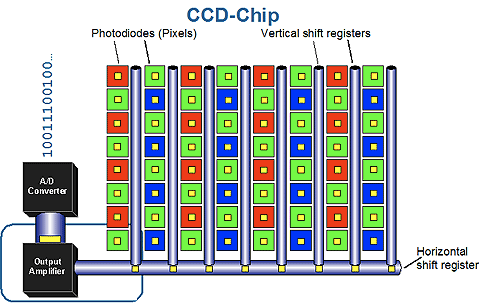
\includegraphics[width=6cm]{ccd}
\caption{Arquitectura base de un sensor CCD.}
\label{sensor_ccd}
\end{figure}

Este tipo de sensores es utilizado en cámara de alto desempe\~no como por ejemplo satélites, cámaras profesionales, telescopios, etc.

\section{\textbf{Tecnologías CCD}}
 
\subsection{\textbf{Transferencia Interlinea (Interline Transfer)}}

Esta arquitectura trata de compensar la mayoría de las deficiencias presentadas al momento en que se da la transferencia de los píxeles. Dise\~nada con una estructura híbrida, con un foto-diodo y un arreglo CCD como lo muestra la figura \ref{il_ccd}. 

\begin{figure}[H]
\centering
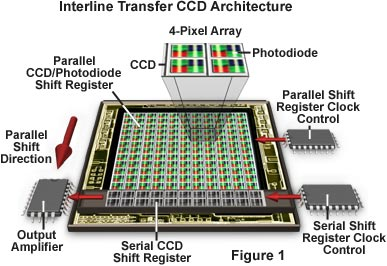
\includegraphics[width=6cm]{interlineccd}
\caption{Tecnología Interline Transfer \cite{IL_CCD1}.}
\label{il_ccd}
\end{figure}

El eje vertical del CCD es atravesado por los elementos del foto-diodo, los cuales comprenden el plano de la imagen y recogen los fotones entrantes proyectados en la superficie del CCD. Una vez se convierten en potencial eléctrico son transferidos al área paralela de CCD adyacente de cada elemento de píxel.

De las mayores ventajas de esta arquitectura es que no no se necesita un obturador o estroboscopio sincronizado, lo que permite un aumento en la velocidad del dispositivo y velocidades de cuadro más rápidas. Dada la tasa de transferencia de imagen alta, en comparación con otras arquitecturas  (i.e. arquitectura de transferencia de trama), se reduce el problema del refrescamiento de imagen. La mayor limitante de esta tecnología es que tiene una mayor complejidad en cuanto a su implementación y una menor sensibilidad debido a la disminución del área fotosensible en cada píxel, sin embargo, este problema es resuelto parcialmente con la adición de microlentes para aumentar la cantidad de luz que ingresa a cada elemento \cite{IL_CCD1}.

\subsection{\textbf{Transferencia de Cuadro (Frame Transfer)}}
Esta arquitectura posee un registro de desplazamiento paralelo que se divide en dos áreas separadas y casi idénticas, denominadas matrices de Imagen y Almacenamiento.

\begin{figure}[H]
\centering
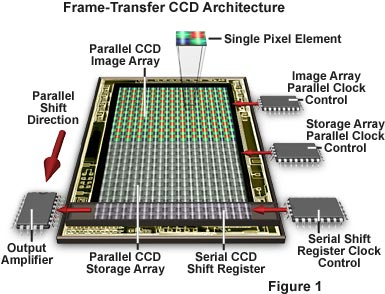
\includegraphics[width=6cm]{ft_ccd}
\caption{Tecnología Frame Transfer \cite{ft_ccd}.}
\label{ft_ccd}
\end{figure}

La matriz de imagen es la encargada de capturar la luz/fotones proyectados en la superficie del CCD por la cámara, este lo convierte a potencial eléctrico y posteriormente se transfieren de forma paralela a la matriz de almacenamiento como se observa en la figura \ref{ft_ccd}. Posteriormente, se da la lectura por medio del registro de desplazamiento serie.

Con el uso de un obturador mecánico, se puede usar un CCD de transferencia de cuadros para capturar rápidamente dos imágenes secuenciales, una característica útil en microscopía de fluorescencia y otras aplicaciones que requieren la adquisición simultánea de imágenes generadas a diferentes longitudes de onda de emisión y o excitación\cite{ft_ccd}.

\subsection{ \textbf{Cuadro Completo (Full Frame)}}
La figura 4 muestra la arquitectura Full Frame, que consiste en un registro de desplazamiento paralelo, sobre el cual se proyectan las imágenes por medio de lentes de cámara o tren óptico de microscopio. Bajo esta configuración, todos los fotodiodos actúan colectivamente y están disponibles para detectar fotones durante el periodo de exposición de luz. Cada píxel consta de cuatro fotodiodos enmascarados con filtros de color rojo, verde y azul como se observa en la figura \ref{fft_ccd}. Después que cada fotón capturado es convertido a potencial eléctrico, se inicia la transferencia paralela, una fila a la vez, hacia el registro de desplazamiento en serie para continuar con el proceso antes explicado\cite{andor}.

Esta arquitectura tiene un factor de relleno del 100\%, lo que significa que toda la matriz de pixeles se usa para detectar fotones entrantes durante la exposicion. Estas matrices por lo general tienen tama\~nos basados en potencias 2 (por ejemplo 512x512, 1024x1024, etc), con el fin de simplificar la asignacion de memoria por parte del los algoritmos de procesamiento de imagenes. Debido al hecho de que el conjunto de píxeles se utiliza tanto para la detección de imágenes como para la lectura, se debe utilizar un obturador mecánico o un esquema de iluminación estroboscópica sincronizada para evitar manchas durante la mayoría de los períodos de exposición. El borrado se produce cuando los fotodiodos se iluminan continuamente durante la lectura del registro paralelo y se orientarán en el sentido del transporte de carga a través de la matriz paralela \cite{fft_ccd}.


\begin{figure}[H]
\centering
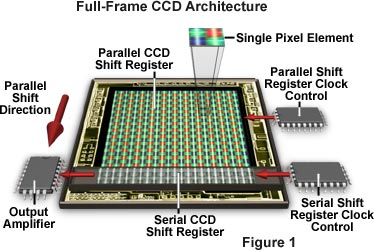
\includegraphics[width=6cm]{fullframeccd}
\caption{Tecnología Full Frame Transfer \cite{fft_ccd}.}
\label{fft_ccd}
\end{figure}


\section{\textbf{Sensor CMOS}}

El sensor CMOS al igual que el CCD se basa en una matriz de fotodiodos que capturan la luz cuando esta incide sobre ellos y posteriormente la convierte en potencial eléctrico. Al ser implementada con tecnología CMOS, cada uno de los píxeles tiene un amplificador por lo que realiza el procesamiento de amplificado de forma mas local y rápida en comparación con los sensores CCD. Posterior a esto la información amplificada, es enviada a través del canal de lectura al convertidor A/D para su posterior almacenamiento en el dispositivo (cámara). La figura \ref{cmos_sensor} muestra una ejemplo de como se vería un sensor CMOS, donde se tienen las diferentes cuadrillas de píxeles y los canales que comunican con el convertidor A/D.

\begin{figure}[H]
\centering
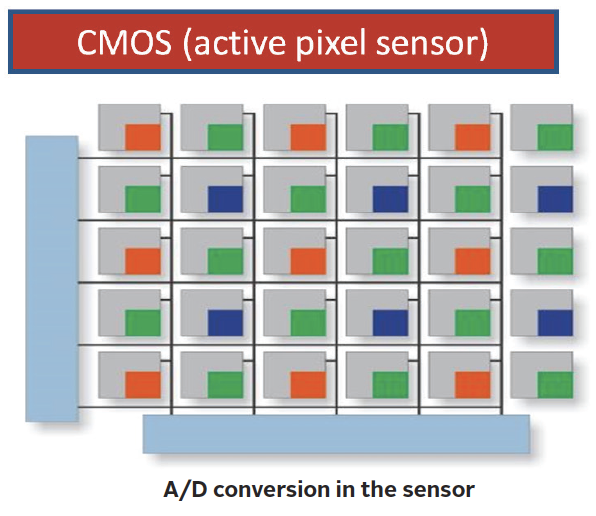
\includegraphics[width=6cm]{cmos_sensor}
\caption{Arquitectura básica de un sensor CMOS \cite{cmos}.}
\label{cmos_sensor}
\end{figure}

Incluso, en implementaciones actuales de sensores CMOS, cada píxel tiene su propio amplificador, corrector de ruido y conversor A/D; por lo que la salida proporcionada va a ser digital, ayudando a que las velocidades de estos sensores sean bastante grandes \cite{ccd_vs_cmos_1}.

\section{\textbf{Ventajas y desventajas de tecnologías CCD contra CMOS.}}
\begin{list}{--}{}
\item
Sensores CCD crean imágenes en alta calidad y con bajo ruido. CMOS es mas susceptible al ruido.
\item
Dado que la densidad de transistores es mayor en el CMOS, mucha de la luz que ingresa al sensor choca contra los transistores y no en el fotodiodo; reduciendo así su capacidad de sensitividad a la luz.
\item
CMOS consume mucha menos potencia (hasta 100 veces menos que un CCD), por lo que lo hace ideal para integrar en productos peque\~nos como teléfonos celulares.
\item
CMOS es mucho mas barato de fabricar que CCD.
\item
Rango dinámico de los sensores CCD es mucho mayor que el de sensores CMOS. 
\end{list}

\section{\textbf{Captura del color}}

\subsection{\textbf{Filtros de Bayer}}
Los sensores de las cámaras no son capaces por si mismos de captar los colores de la imagen que están tratando de capturar como se puede observar en la figura \ref{no_filter_cavity}, mientras que la figura \ref{fotodiodo_sin_filtro} muestra como los ases de luz ingresan al fotodiodo sin ningún tipo de filtrado. Ahora bien, al agregar un filtro a cada uno de los píxeles como lo observado en la figura \ref{fotodiodo_con_filtro}, donde se puede observar como la luz incidente va a ser reflejada si no esta en la longitud de onda que permite el filtro. Una vez aplicado este filtrado de color, se obtiene algo similar a lo mostrado en la figura \ref{filtered_cavity}, donde se obtendría una imagen a color. El proceso antes descrito es lo que se conoce como Filtro de Bayer (llamado así por su autor: Bryce Bayer), donde además, se debe destacar que este filtrado tiene una proporción de 1:2:1 o mejor dicho, 2 verdes por cada 1 rojo y 1 azul (colores primarios) debido a que el ojo humano es mas sensible a los colores verdes\cite{bayer2}.

\begin{figure}[H]
    \centering
    \begin{subfigure}[b]{3cm}
        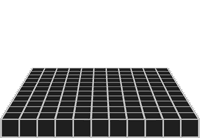
\includegraphics[width=\textwidth]{bayer1}
        \caption{Sensor sin filtro de color}
        \label{no_filter_cavity}
    \end{subfigure}
    ~ %add desired spacing between images, e. g. ~, \quad, \qquad, \hfill etc. 
      %(or a blank line to force the subfigure onto a new line)
    \begin{subfigure}[b]{3cm}
        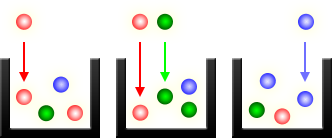
\includegraphics[width=\textwidth]{bayer2}
        \caption{Fotodiodo sin filtro de color}
        \label{fotodiodo_sin_filtro}
    \end{subfigure}
    ~ %add desired spacing between images, e. g. ~, \quad, \qquad, \hfill etc. 
    %(or a blank line to force the subfigure onto a new line)
    \begin{subfigure}[b]{3cm}
        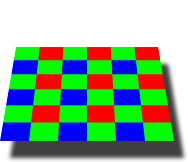
\includegraphics[width=\textwidth]{bayer3}
        \caption{Sensor con filtro de color}
        \label{filtered_cavity}
    \end{subfigure}
    ~ %add desired spacing between images, e. g. ~, \quad, \qquad, \hfill etc. 
    %(or a blank line to force the subfigure onto a new line)
    \begin{subfigure}[b]{3cm}
        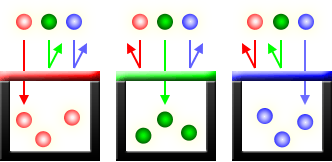
\includegraphics[width=\textwidth]{bayer}
        \caption{Fotodiodo con filtro de color}
        \label{fotodiodo_con_filtro}
    \end{subfigure}
    \caption{Filtro Bayer\cite{bayer}}\label{filtro_bayer}
\end{figure}

Posterior a la captura se debe aplicar el \'Bayer Demosaicing\', que consiste en llevar a la imagen de solamente tener colores en un arreglo de colores primarios a una imagen que contenga la información completa del color de cada píxel.

\subsection{\textbf{Sensores Foveon X3}}
El Foveon X3 es un sensor que captura directamente la luz color rojo, verde y azul presente en una imagen durante un única exposición. En la figura \ref{x3} se muestra el funcionamiento de este sensor, que aprovecha el hecho de que la luz penetra con diferente profundidad el silicio para que cada píxel tenga la capacidad de tener una captura completa del color en cada punto de la imagen.  

\begin{figure}[H]
\centering
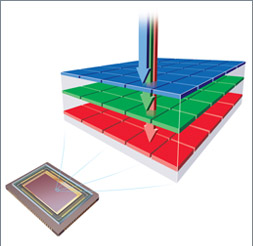
\includegraphics[width=6cm]{x3}
\caption{Foveon X3 \cite{foveon}.}
\label{x3}
\end{figure}

Este tipo de tecnologías ayudaran a que se puedan crear cámaras que no discriminen en calidad cuando se hacen cambios de modo entre imagen y grabar vídeo \cite{foveon}.

\subsection{\textbf{C\'amaras de Triple CCD}}
Este tipo de cámaras utilizan un prisma dicroico que, al as de luz incidente, lo divide en tres diferente canales de color (rojo, verde y azul), tal y como se puede observar en la figura \ref{3ccd}. Con este proceso de división de color, se van a tener valores RGB de alta precision por lo que ayudara a tener una alta fidelidad de color, alto rango dinámico y cámaras con la capacidad de contener algoritmos especializados para la calibración del espacio de color \cite{3ccd}.

\begin{figure}[H]
\centering
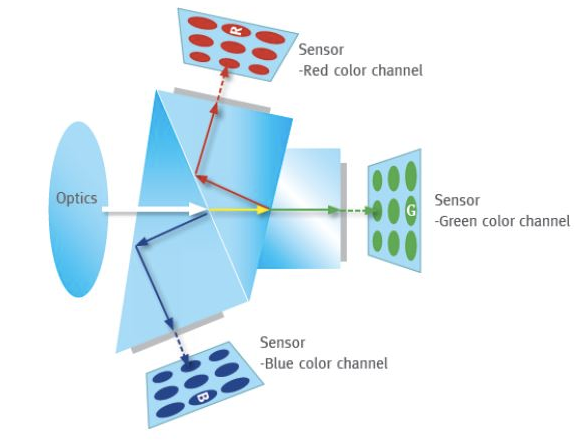
\includegraphics[width=6cm]{3ccd}
\caption{Principio de funcionamiento de las Cámaras con triple CCD \cite{3ccd}.}
\label{3ccd}
\end{figure}


\bibliographystyle{IEEEtran}
\bibliography{bibliografia}

%


% that's all folks
\end{document}





